% Options for packages loaded elsewhere
\PassOptionsToPackage{unicode}{hyperref}
\PassOptionsToPackage{hyphens}{url}
%
\documentclass[
]{article}
\usepackage{amsmath,amssymb}
\usepackage{iftex}
\ifPDFTeX
  \usepackage[T1]{fontenc}
  \usepackage[utf8]{inputenc}
  \usepackage{textcomp} % provide euro and other symbols
\else % if luatex or xetex
  \usepackage{unicode-math} % this also loads fontspec
  \defaultfontfeatures{Scale=MatchLowercase}
  \defaultfontfeatures[\rmfamily]{Ligatures=TeX,Scale=1}
\fi
\usepackage{lmodern}
\ifPDFTeX\else
  % xetex/luatex font selection
\fi
% Use upquote if available, for straight quotes in verbatim environments
\IfFileExists{upquote.sty}{\usepackage{upquote}}{}
\IfFileExists{microtype.sty}{% use microtype if available
  \usepackage[]{microtype}
  \UseMicrotypeSet[protrusion]{basicmath} % disable protrusion for tt fonts
}{}
\makeatletter
\@ifundefined{KOMAClassName}{% if non-KOMA class
  \IfFileExists{parskip.sty}{%
    \usepackage{parskip}
  }{% else
    \setlength{\parindent}{0pt}
    \setlength{\parskip}{6pt plus 2pt minus 1pt}}
}{% if KOMA class
  \KOMAoptions{parskip=half}}
\makeatother
\usepackage{xcolor}
\usepackage[margin=1in]{geometry}
\usepackage{color}
\usepackage{fancyvrb}
\newcommand{\VerbBar}{|}
\newcommand{\VERB}{\Verb[commandchars=\\\{\}]}
\DefineVerbatimEnvironment{Highlighting}{Verbatim}{commandchars=\\\{\}}
% Add ',fontsize=\small' for more characters per line
\usepackage{framed}
\definecolor{shadecolor}{RGB}{248,248,248}
\newenvironment{Shaded}{\begin{snugshade}}{\end{snugshade}}
\newcommand{\AlertTok}[1]{\textcolor[rgb]{0.94,0.16,0.16}{#1}}
\newcommand{\AnnotationTok}[1]{\textcolor[rgb]{0.56,0.35,0.01}{\textbf{\textit{#1}}}}
\newcommand{\AttributeTok}[1]{\textcolor[rgb]{0.13,0.29,0.53}{#1}}
\newcommand{\BaseNTok}[1]{\textcolor[rgb]{0.00,0.00,0.81}{#1}}
\newcommand{\BuiltInTok}[1]{#1}
\newcommand{\CharTok}[1]{\textcolor[rgb]{0.31,0.60,0.02}{#1}}
\newcommand{\CommentTok}[1]{\textcolor[rgb]{0.56,0.35,0.01}{\textit{#1}}}
\newcommand{\CommentVarTok}[1]{\textcolor[rgb]{0.56,0.35,0.01}{\textbf{\textit{#1}}}}
\newcommand{\ConstantTok}[1]{\textcolor[rgb]{0.56,0.35,0.01}{#1}}
\newcommand{\ControlFlowTok}[1]{\textcolor[rgb]{0.13,0.29,0.53}{\textbf{#1}}}
\newcommand{\DataTypeTok}[1]{\textcolor[rgb]{0.13,0.29,0.53}{#1}}
\newcommand{\DecValTok}[1]{\textcolor[rgb]{0.00,0.00,0.81}{#1}}
\newcommand{\DocumentationTok}[1]{\textcolor[rgb]{0.56,0.35,0.01}{\textbf{\textit{#1}}}}
\newcommand{\ErrorTok}[1]{\textcolor[rgb]{0.64,0.00,0.00}{\textbf{#1}}}
\newcommand{\ExtensionTok}[1]{#1}
\newcommand{\FloatTok}[1]{\textcolor[rgb]{0.00,0.00,0.81}{#1}}
\newcommand{\FunctionTok}[1]{\textcolor[rgb]{0.13,0.29,0.53}{\textbf{#1}}}
\newcommand{\ImportTok}[1]{#1}
\newcommand{\InformationTok}[1]{\textcolor[rgb]{0.56,0.35,0.01}{\textbf{\textit{#1}}}}
\newcommand{\KeywordTok}[1]{\textcolor[rgb]{0.13,0.29,0.53}{\textbf{#1}}}
\newcommand{\NormalTok}[1]{#1}
\newcommand{\OperatorTok}[1]{\textcolor[rgb]{0.81,0.36,0.00}{\textbf{#1}}}
\newcommand{\OtherTok}[1]{\textcolor[rgb]{0.56,0.35,0.01}{#1}}
\newcommand{\PreprocessorTok}[1]{\textcolor[rgb]{0.56,0.35,0.01}{\textit{#1}}}
\newcommand{\RegionMarkerTok}[1]{#1}
\newcommand{\SpecialCharTok}[1]{\textcolor[rgb]{0.81,0.36,0.00}{\textbf{#1}}}
\newcommand{\SpecialStringTok}[1]{\textcolor[rgb]{0.31,0.60,0.02}{#1}}
\newcommand{\StringTok}[1]{\textcolor[rgb]{0.31,0.60,0.02}{#1}}
\newcommand{\VariableTok}[1]{\textcolor[rgb]{0.00,0.00,0.00}{#1}}
\newcommand{\VerbatimStringTok}[1]{\textcolor[rgb]{0.31,0.60,0.02}{#1}}
\newcommand{\WarningTok}[1]{\textcolor[rgb]{0.56,0.35,0.01}{\textbf{\textit{#1}}}}
\usepackage{graphicx}
\makeatletter
\def\maxwidth{\ifdim\Gin@nat@width>\linewidth\linewidth\else\Gin@nat@width\fi}
\def\maxheight{\ifdim\Gin@nat@height>\textheight\textheight\else\Gin@nat@height\fi}
\makeatother
% Scale images if necessary, so that they will not overflow the page
% margins by default, and it is still possible to overwrite the defaults
% using explicit options in \includegraphics[width, height, ...]{}
\setkeys{Gin}{width=\maxwidth,height=\maxheight,keepaspectratio}
% Set default figure placement to htbp
\makeatletter
\def\fps@figure{htbp}
\makeatother
\setlength{\emergencystretch}{3em} % prevent overfull lines
\providecommand{\tightlist}{%
  \setlength{\itemsep}{0pt}\setlength{\parskip}{0pt}}
\setcounter{secnumdepth}{-\maxdimen} % remove section numbering
\ifLuaTeX
  \usepackage{selnolig}  % disable illegal ligatures
\fi
\IfFileExists{bookmark.sty}{\usepackage{bookmark}}{\usepackage{hyperref}}
\IfFileExists{xurl.sty}{\usepackage{xurl}}{} % add URL line breaks if available
\urlstyle{same}
\hypersetup{
  pdftitle={Correspondance entre classes étiquettées et Clusters prédits par algorithme hongrois},
  pdfauthor={Willy Kinfoussia, Aurélien Henriques},
  hidelinks,
  pdfcreator={LaTeX via pandoc}}

\title{Correspondance entre classes étiquettées et Clusters prédits par
algorithme hongrois}
\author{Willy Kinfoussia, Aurélien Henriques}
\date{2023-2024 M2DS}

\begin{document}
\maketitle

\hypertarget{section}{%
\subsection{}\label{section}}

Introduction

Un problème notable dans l'apprentissage supervisé est la labélisation
d'un grand nombre de données afin d'entraîner un modèle. En effet, Il
arrive souvent que le nombre de données labelisées soit dérisoire
comparément aux données dont l'on dispose au total. Certains
algorithmes, par exemple l'algorithme SWAV, permettent de s'affranchir
de ce problème en créant une représentation de classe par alteration
faible des exemples labélisés, mais ils nécessitent un apprentissage
contrastif afin de pouvoir identifier une classe.

Les algorithmes de clusterisation non-supervisé peuvent alors permettre
de résoudre ce problème, en clusterisant les données par cluster pourvu
que nous puissions identifier correctement les clusters aux étiquettes
de classe. Dans ce cas, il suffirait alors de s'assurer de la bonne
représentation du modèle des différentes classes via les clusters, et
d'apposer aux données des clusters les étiquettes de classe issue de
l'association cluster/classe.

\hypertarget{section-1}{%
\subsection{}\label{section-1}}

Dans ce projet, nous proposons d'appliquer l'algorithme hongrois à ce
problème. L'algorithme hongrois est un programme qui permet de trouver
la meilleure association entre N agents et N tâches à l'aide de poids
associés aux arrêtes entre agents et tâches. En pratique, il existe N**2
poids d'arrête et N ! façons différentes d'associer les agents aux
tâches. La recherche de l'optimum des associations peut donc être
pénible et utiliser l'algorithme hongrois permet de résoudre en partie
ce problème, grâce une complexité polynômiale en N. Il repose sur une
recherche du poids d'arrête minimal dans une matrice de coût qui
contiendrait tous les poids des arrêtes entre agents et tâches (dans
notre cas, entre cluster et classe). Nous utilisons ici cet algorithme
ainsi qu'un algorithme naîf parcourant les N! possibilités

\hypertarget{section-2}{%
\subsection{}\label{section-2}}

Construction de la matrice de coût

Nous collectons les données MNIST, ainsi que les classes associées pour
obtenir une matrice de coût. Pour ceci, nous effectuons une PCA à 50
dimensions sur les données puis nous clusterisons par k-nn les données
obtenues en 10 clusters (le nombre de classe dans MNIST). Nous calculons
alors les centres d'inertie des classes et des clusters puis l'on
utilise la distance euclidienne entre chaque couple classe/cluster.

\[
\text{d}(c, k) = \sqrt{\sum_{l=1}^{50} (c_{l} - k_{l})^2}
\]

Où : - \(c_l\) représente la valeur du centre d'inertie de la classe
\(c\) en la l-ème dimension, - \(k_l\) représente la valeur du centre
d'inertie du cluster \(k\) en la l-ème dimension,

\hypertarget{section-3}{%
\subsection{}\label{section-3}}

\begin{Shaded}
\begin{Highlighting}[]
\NormalTok{mnist\_train }\OtherTok{\textless{}{-}}  \FunctionTok{read.csv}\NormalTok{(}\StringTok{\textquotesingle{}mnist\_test.csv\textquotesingle{}}\NormalTok{)}

\NormalTok{x\_train }\OtherTok{\textless{}{-}}\NormalTok{ mnist\_train[, }\SpecialCharTok{{-}}\DecValTok{1}\NormalTok{]}
\NormalTok{y\_train }\OtherTok{\textless{}{-}}\NormalTok{ mnist\_train[, }\DecValTok{1}\NormalTok{]}

\NormalTok{x\_train\_vec }\OtherTok{\textless{}{-}}\NormalTok{ x\_train }\SpecialCharTok{/} \DecValTok{255}

\NormalTok{constant\_columns }\OtherTok{\textless{}{-}} \FunctionTok{apply}\NormalTok{(x\_train\_vec, }\DecValTok{2}\NormalTok{, }\ControlFlowTok{function}\NormalTok{(col) }\FunctionTok{length}\NormalTok{(}\FunctionTok{unique}\NormalTok{(col)) }\SpecialCharTok{==} \DecValTok{1}\NormalTok{)}
\NormalTok{x\_train\_vec }\OtherTok{\textless{}{-}}\NormalTok{ x\_train\_vec[, }\SpecialCharTok{!}\NormalTok{constant\_columns]}

\NormalTok{pca }\OtherTok{\textless{}{-}} \FunctionTok{prcomp}\NormalTok{(x\_train\_vec, }\AttributeTok{center =} \ConstantTok{TRUE}\NormalTok{, }\AttributeTok{scale. =} \ConstantTok{TRUE}\NormalTok{, }\AttributeTok{rank =} \DecValTok{50}\NormalTok{)}

\NormalTok{x\_train\_pca }\OtherTok{\textless{}{-}} \FunctionTok{predict}\NormalTok{(pca, x\_train\_vec)}
\end{Highlighting}
\end{Shaded}

\hypertarget{section-4}{%
\subsection{}\label{section-4}}

\begin{Shaded}
\begin{Highlighting}[]
\FunctionTok{library}\NormalTok{(stats)}

\NormalTok{k }\OtherTok{\textless{}{-}} \DecValTok{10}

\NormalTok{kmeans\_model }\OtherTok{\textless{}{-}} \FunctionTok{kmeans}\NormalTok{(x\_train\_pca, }\AttributeTok{centers =}\NormalTok{ k)}

\NormalTok{clusters\_centroid }\OtherTok{\textless{}{-}}\NormalTok{ kmeans\_model}\SpecialCharTok{$}\NormalTok{centers}

\NormalTok{assignement\_cluster }\OtherTok{\textless{}{-}}\NormalTok{ kmeans\_model}\SpecialCharTok{$}\NormalTok{cluster}

\NormalTok{classes\_centroid }\OtherTok{\textless{}{-}} \FunctionTok{list}\NormalTok{()}
\end{Highlighting}
\end{Shaded}

\hypertarget{section-5}{%
\subsection{}\label{section-5}}

Optimisation

La matrice de coût est alors :

\[
\text{M} = (d_{ck}) 
\]

Où : - c et k varient entre 1 et 10.

La matrice \(X\) d'association classe/cluster de taille \((10,10)\) est
définie comme :

\[
X_{ck} = 
\begin{cases} 
1 & \text{si la classe } c \text{ et le cluster } k \text{ sont associés} \\
0 & \text{sinon} 
\end{cases}
\]

avec la contrainte qu'il ne doit y avoir qu'un seul \(1\) par ligne et
des \(0\) sur le reste, correspondant à ne pas associer la classe c aux
autres clusters.

\[
\ \sum_{k=1}^{10} X_{ck} = 1
\]

\hypertarget{section-6}{%
\subsection{}\label{section-6}}

\begin{Shaded}
\begin{Highlighting}[]
\ControlFlowTok{for}\NormalTok{ (class\_label }\ControlFlowTok{in} \DecValTok{0}\SpecialCharTok{:}\NormalTok{(k }\SpecialCharTok{{-}} \DecValTok{1}\NormalTok{)) \{}
  
\NormalTok{  class\_data }\OtherTok{\textless{}{-}}\NormalTok{ x\_train\_pca[y\_train }\SpecialCharTok{==}\NormalTok{ class\_label, ]}
  
\NormalTok{  centroid }\OtherTok{\textless{}{-}} \FunctionTok{colMeans}\NormalTok{(class\_data)}
  
\NormalTok{  classes\_centroid[[}\FunctionTok{as.character}\NormalTok{(class\_label)]] }\OtherTok{\textless{}{-}}\NormalTok{ centroid}
\NormalTok{\}}

\NormalTok{cost\_matrix\_mnist }\OtherTok{\textless{}{-}} \FunctionTok{matrix}\NormalTok{(}\DecValTok{0}\NormalTok{, }\AttributeTok{nrow =}\NormalTok{ k, }\AttributeTok{ncol =}\NormalTok{ k)}

\ControlFlowTok{for}\NormalTok{ (i }\ControlFlowTok{in} \DecValTok{0}\SpecialCharTok{:}\NormalTok{k}\DecValTok{{-}1}\NormalTok{) \{}
  \ControlFlowTok{for}\NormalTok{ (j }\ControlFlowTok{in} \DecValTok{1}\SpecialCharTok{:}\NormalTok{k) \{}

\NormalTok{    distance }\OtherTok{\textless{}{-}} \FunctionTok{sqrt}\NormalTok{(}\FunctionTok{sum}\NormalTok{((classes\_centroid[[}\FunctionTok{as.character}\NormalTok{(i)]] }\SpecialCharTok{{-}}\NormalTok{ clusters\_centroid[j, ])}\SpecialCharTok{\^{}}\DecValTok{2}\NormalTok{))}
    
\NormalTok{    cost\_matrix\_mnist[i}\SpecialCharTok{+}\DecValTok{1}\NormalTok{, j] }\OtherTok{\textless{}{-}}\NormalTok{ distance}
\NormalTok{  \}}
\NormalTok{\}}

\NormalTok{cost\_matrix\_mnist }\OtherTok{\textless{}{-}} \FunctionTok{lapply}\NormalTok{(}\DecValTok{1}\SpecialCharTok{:}\NormalTok{k, }\ControlFlowTok{function}\NormalTok{(i) }\FunctionTok{as.vector}\NormalTok{(cost\_matrix\_mnist[i, ]))}
\end{Highlighting}
\end{Shaded}

\hypertarget{section-7}{%
\subsection{}\label{section-7}}

\begin{Shaded}
\begin{Highlighting}[]
\CommentTok{\#Génération de matrice de coût aléatoire}

\NormalTok{matrice\_couts }\OtherTok{\textless{}{-}} \ControlFlowTok{function}\NormalTok{(n) \{}
  
\NormalTok{  cost\_matrix\_random }\OtherTok{\textless{}{-}} \FunctionTok{matrix}\NormalTok{(}\FunctionTok{rnorm}\NormalTok{(n }\SpecialCharTok{*}\NormalTok{ n, }\AttributeTok{mean =} \DecValTok{100}\NormalTok{, }\AttributeTok{sd =} \DecValTok{15}\NormalTok{), }\AttributeTok{nrow =}\NormalTok{ n, }\AttributeTok{ncol =}\NormalTok{ n)}
\NormalTok{  liste\_matrice }\OtherTok{\textless{}{-}} \FunctionTok{lapply}\NormalTok{(}\DecValTok{1}\SpecialCharTok{:}\NormalTok{n, }\ControlFlowTok{function}\NormalTok{(i) }\FunctionTok{as.vector}\NormalTok{(cost\_matrix\_random[i, ]))}
  
  \FunctionTok{return}\NormalTok{(liste\_matrice)}
\NormalTok{\}}
\end{Highlighting}
\end{Shaded}

\hypertarget{section-8}{%
\subsection{}\label{section-8}}

Comme on souhaite aussi qu'un cluster corresponde à une ligne (
éventuellement il est possible de faire concorder plusieurs clusters à
une classe et inversement en enlevant les contraintes sur la bijection
de notre association), une seconde contrainte est qu'il ne doit y avoir
qu'un 1 par ligne et des 0 sur le reste.

\[
\ \sum_{c=1}^{10} X_{ck} = 1
\]

La fonction de coût à minimiser est la somme des produits
\(X_{kl} \times M_{kl}\) sur \(l\) et \(k\) :

\[
\text{Coût(association X)} = \sum_{c=1}^{10} \sum_{k=1}^{10} X_{ck} \times M_{ck}
\]

Cette fonction correspond au coût de l'association classe/cluster
choisie. En la minimisant, on s'assure que l'association permet au
maximum de réduire la distance séparant le cluster de la classe.

\hypertarget{section-9}{%
\subsection{}\label{section-9}}

Algorithme naîf

L'algorithme naîf permet de résoudre ce problème brutalement en
calculant toutes les coûts possibles. C'est-à-dire calculer pour chaque
bijection classes-cluster la somme des arrêtes associant un cluster à
une classe et renvoyer la bijection qui minimise le coût. La complexité
théorique de cet algorithmique est N! où N est le nombre de
classes/clusters. En effet, pour la classe 1, il y a 10 clusters
possibles. Une fois un cluster choisi, on obtient le premier coefficient
de coût. Il reste donc pour la classe 2 9 clusters possibles, 8 pour la
classe 3, etc. Ceci donne bien N! associations possibles donc N! somme
des coûts possibles, ce qui donne la complexité de cet algorithme.

\hypertarget{section-10}{%
\subsection{}\label{section-10}}

\begin{Shaded}
\begin{Highlighting}[]
\FunctionTok{library}\NormalTok{(Rcpp)}
\end{Highlighting}
\end{Shaded}

\begin{verbatim}
## Warning: le package 'Rcpp' a été compilé avec la version R 4.3.3
\end{verbatim}

\begin{Shaded}
\begin{Highlighting}[]
\FunctionTok{sourceCpp}\NormalTok{(}\StringTok{"NaiveAlgorithme.cpp"}\NormalTok{)}
\end{Highlighting}
\end{Shaded}

\hypertarget{section-11}{%
\subsection{}\label{section-11}}

Complexité expérimentale

\begin{Shaded}
\begin{Highlighting}[]
\NormalTok{temps\_execution }\OtherTok{\textless{}{-}} \ControlFlowTok{function}\NormalTok{(n\_liste,p,algo) \{}

\NormalTok{  temps }\OtherTok{\textless{}{-}} \FunctionTok{numeric}\NormalTok{(}\FunctionTok{length}\NormalTok{(n\_liste))}
  
  \ControlFlowTok{for}\NormalTok{ (j }\ControlFlowTok{in} \FunctionTok{seq\_along}\NormalTok{(n\_liste)) \{}
\NormalTok{    n }\OtherTok{\textless{}{-}}\NormalTok{ n\_liste[j]}
\NormalTok{    cout }\OtherTok{\textless{}{-}} \FunctionTok{matrice\_couts}\NormalTok{(n)}
    
\NormalTok{    start\_time }\OtherTok{\textless{}{-}} \FunctionTok{Sys.time}\NormalTok{()}
    
    \ControlFlowTok{for}\NormalTok{ (i }\ControlFlowTok{in} \DecValTok{0}\SpecialCharTok{:}\NormalTok{(p}\DecValTok{{-}1}\NormalTok{)) \{}
    \FunctionTok{algo}\NormalTok{(cout)}
\NormalTok{    \}}
    
\NormalTok{    end\_time }\OtherTok{\textless{}{-}} \FunctionTok{Sys.time}\NormalTok{()}
\NormalTok{    temps[j] }\OtherTok{\textless{}{-}}\NormalTok{ (end\_time }\SpecialCharTok{{-}}\NormalTok{ start\_time)}\SpecialCharTok{/}\NormalTok{p}
\NormalTok{  \}}
  \FunctionTok{return}\NormalTok{(temps)}
\NormalTok{\}}
\end{Highlighting}
\end{Shaded}

\hypertarget{section-12}{%
\subsection{}\label{section-12}}

Pour obtenir la complexité, on détermine la régression
log(T)=f(n*log(n)-n) où l'on a utilisé la formule de stirling par
simplicité:

\begin{Shaded}
\begin{Highlighting}[]
\NormalTok{liste\_dimension }\OtherTok{\textless{}{-}} \FunctionTok{seq}\NormalTok{(}\AttributeTok{from =} \DecValTok{5}\NormalTok{, }\AttributeTok{to =} \DecValTok{12}\NormalTok{, }\AttributeTok{by =} \DecValTok{1}\NormalTok{)}

\NormalTok{logn\_n }\OtherTok{\textless{}{-}}\NormalTok{ (}\FunctionTok{log}\NormalTok{(liste\_dimension)}\SpecialCharTok{{-}}\DecValTok{1}\NormalTok{)}\SpecialCharTok{*}\NormalTok{liste\_dimension}

\NormalTok{temps\_exe }\OtherTok{\textless{}{-}} \FunctionTok{log}\NormalTok{(}\FunctionTok{temps\_execution}\NormalTok{(liste\_dimension,}\DecValTok{5}\NormalTok{,NaiveAlgorithme)) }

\FunctionTok{plot}\NormalTok{(}\FunctionTok{log}\NormalTok{(liste\_dimension),temps\_exe,}\AttributeTok{xlab=}\StringTok{\textquotesingle{}log(nombre de classes)\textquotesingle{}}\NormalTok{,}\AttributeTok{ylab=}\StringTok{\textquotesingle{}log(temps)\textquotesingle{}}\NormalTok{)}
\end{Highlighting}
\end{Shaded}

\includegraphics{main_files/figure-latex/unnamed-chunk-7-1.pdf}

\begin{Shaded}
\begin{Highlighting}[]
\NormalTok{reg }\OtherTok{\textless{}{-}} \FunctionTok{lm}\NormalTok{(temps\_exe}\SpecialCharTok{\textasciitilde{}}\NormalTok{logn\_n)}

\FunctionTok{summary}\NormalTok{(reg)}
\end{Highlighting}
\end{Shaded}

\begin{verbatim}
## 
## Call:
## lm(formula = temps_exe ~ logn_n)
## 
## Residuals:
##     Min      1Q  Median      3Q     Max 
## -1.6632 -0.8322 -0.1471  0.4174  2.7435 
## 
## Coefficients:
##             Estimate Std. Error t value Pr(>|t|)    
## (Intercept) -13.2945     1.1986 -11.092  3.2e-05 ***
## logn_n        0.8250     0.1077   7.657 0.000259 ***
## ---
## Signif. codes:  0 '***' 0.001 '**' 0.01 '*' 0.05 '.' 0.1 ' ' 1
## 
## Residual standard error: 1.481 on 6 degrees of freedom
## Multiple R-squared:  0.9072, Adjusted R-squared:  0.8917 
## F-statistic: 58.62 on 1 and 6 DF,  p-value: 0.0002594
\end{verbatim}

\begin{Shaded}
\begin{Highlighting}[]
\FunctionTok{print}\NormalTok{(}\FunctionTok{coef}\NormalTok{(reg)[}\DecValTok{2}\NormalTok{])}
\end{Highlighting}
\end{Shaded}

\begin{verbatim}
##    logn_n 
## 0.8249515
\end{verbatim}

La régression donne des valeurs proches de 1 (0.88-0.94) avec un
R\^{}2\textgreater0.88. Ainsi, on a bien une complexité en N! par
équivalence avec n*log(n)-n.~

\hypertarget{section-13}{%
\subsection{}\label{section-13}}

Algorithme hongrois

Étape 0 : Soustraire le minimum de chaque ligne à tous les éléments de
cette ligne, puis soustraire le minimum de chaque colonne à tous les
éléments de cette colonne dans la matrice de coût.

Étape 1 : Sélectionner le maximum de zéros indépendants, c'est-à-dire un
seul zéro par ligne et par colonne, en parcourant tous les zéros non
sélectionnés et en les sélectionnant s'ils ne partagent pas la même
ligne ou colonne qu'un zéro déjà sélectionné.

Étape 2 : Couvrir chaque colonne ayant un zéro sélectionné. Puis, pour
chaque zéro non couvert, marquer la colonne de ce zéro et couvrir la
ligne de ce zéro si aucune colonne n'est marquée pour ce zéro. Répéter
jusqu'à ce qu'il n'y ait plus de zéros non couverts.

Étape 3 : Trouver la valeur minimum des éléments non couverts dans la
matrice. Ajouter cette valeur à toutes les lignes couvertes et la
retirer à toutes les colonnes non couvertes. Recommencer à l'étape 1

\hypertarget{section-14}{%
\subsection{}\label{section-14}}

Complexité

Les différentes étapes sont faites avec une complexité de 1 sur la
totalité de la matrice de coût donc ont une complexité maximale de
O(n\^{}2). De plus, Une itération de ces étapes garantit d'avoir au
moins un zéro indépendant, ce qui indique que l'algorithme résout le
problème au maximum en n\^{}2 itérations, correspondant au cas le cas le
plus extrême, à devoir itérer sur chacun des coefficients de la matrice
d'assignation, qui a n\^{}2 coefficients. On en déduit que l'algorithme
a une complexité théorique en O(n\^{}4)

\hypertarget{section-15}{%
\subsection{}\label{section-15}}

\begin{Shaded}
\begin{Highlighting}[]
\FunctionTok{sourceCpp}\NormalTok{(}\StringTok{"Hungarian.cpp"}\NormalTok{)}
\end{Highlighting}
\end{Shaded}

\begin{Shaded}
\begin{Highlighting}[]
\NormalTok{liste\_dimension }\OtherTok{\textless{}{-}} \FunctionTok{seq}\NormalTok{(}\AttributeTok{from =} \DecValTok{10}\NormalTok{, }\AttributeTok{to =} \DecValTok{450}\NormalTok{, }\AttributeTok{by =} \DecValTok{20}\NormalTok{)}

\NormalTok{temps\_exe\_hong }\OtherTok{\textless{}{-}} \FunctionTok{log}\NormalTok{(}\FunctionTok{temps\_execution}\NormalTok{(liste\_dimension,}\DecValTok{5}\NormalTok{,Hungarian))}

\FunctionTok{plot}\NormalTok{(}\FunctionTok{log}\NormalTok{(liste\_dimension),temps\_exe\_hong,}\AttributeTok{xlab=}\StringTok{\textquotesingle{}log(nombre de classes)\textquotesingle{}}\NormalTok{,}\AttributeTok{ylab=}\StringTok{\textquotesingle{}log(temps\textquotesingle{}}\NormalTok{)}
\end{Highlighting}
\end{Shaded}

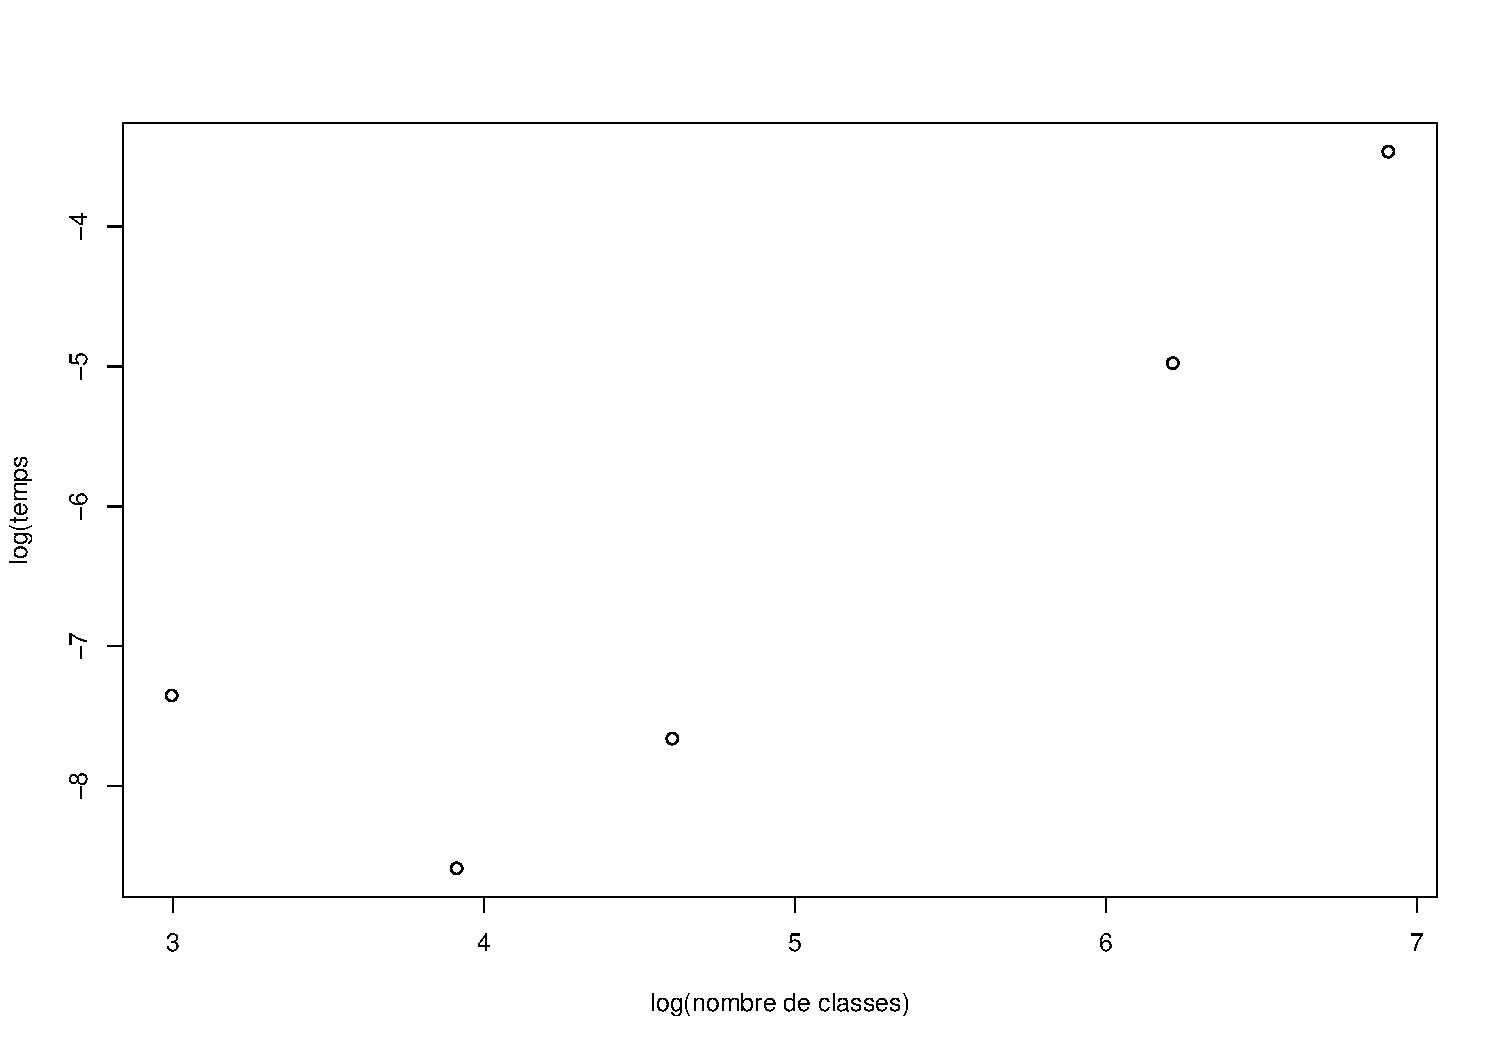
\includegraphics{main_files/figure-latex/unnamed-chunk-9-1.pdf}

\begin{Shaded}
\begin{Highlighting}[]
\NormalTok{reg }\OtherTok{\textless{}{-}} \FunctionTok{lm}\NormalTok{(temps\_exe\_hong}\SpecialCharTok{\textasciitilde{}}\FunctionTok{log}\NormalTok{(liste\_dimension))}

\FunctionTok{summary}\NormalTok{(reg)}
\end{Highlighting}
\end{Shaded}

\begin{verbatim}
## 
## Call:
## lm(formula = temps_exe_hong ~ log(liste_dimension))
## 
## Residuals:
##     Min      1Q  Median      3Q     Max 
## -0.8843 -0.4348 -0.1091  0.3290  2.0364 
## 
## Coefficients:
##                      Estimate Std. Error t value Pr(>|t|)    
## (Intercept)          -15.6956     0.7541  -20.81 1.69e-15 ***
## log(liste_dimension)   2.4387     0.1442   16.91 1.04e-13 ***
## ---
## Signif. codes:  0 '***' 0.001 '**' 0.01 '*' 0.05 '.' 0.1 ' ' 1
## 
## Residual standard error: 0.6448 on 21 degrees of freedom
## Multiple R-squared:  0.9316, Adjusted R-squared:  0.9283 
## F-statistic:   286 on 1 and 21 DF,  p-value: 1.041e-13
\end{verbatim}

\begin{Shaded}
\begin{Highlighting}[]
\FunctionTok{print}\NormalTok{(}\StringTok{"complexité polynomiale :"}\NormalTok{)}
\end{Highlighting}
\end{Shaded}

\begin{verbatim}
## [1] "complexité polynomiale :"
\end{verbatim}

\begin{Shaded}
\begin{Highlighting}[]
\FunctionTok{print}\NormalTok{(}\FunctionTok{coef}\NormalTok{(reg)[}\DecValTok{2}\NormalTok{])}
\end{Highlighting}
\end{Shaded}

\begin{verbatim}
## log(liste_dimension) 
##             2.438655
\end{verbatim}

\hypertarget{section-16}{%
\subsection{}\label{section-16}}

Performances sur MNIST

On utilise les clusters associés aux classes pour prédire le test de
mnist. Pour ce faire, nous utilisons la matrice d'assignation
classe/cluster obtenue pour assigner les classes aux clusters prédits
par l'algorithme des k-means. Nous comparons ensuite avec la vraie
classe des données test mnist avec celle prédite par cette association.

\hypertarget{section-17}{%
\subsection{}\label{section-17}}

\begin{Shaded}
\begin{Highlighting}[]
\NormalTok{assignation }\OtherTok{\textless{}{-}} \FunctionTok{Hungarian}\NormalTok{(cost\_matrix\_mnist) }\CommentTok{\# matrice bijection classes/clusters trouvés par l\textquotesingle{}algorithme hongrois}

\NormalTok{association }\OtherTok{\textless{}{-}}\FunctionTok{numeric}\NormalTok{(k) }\CommentTok{\# version liste de la bijection}

\ControlFlowTok{for}\NormalTok{ (i }\ControlFlowTok{in} \FunctionTok{seq\_along}\NormalTok{(assignation)) \{}
  
\NormalTok{  association[i] }\OtherTok{\textless{}{-}} \FunctionTok{which}\NormalTok{(assignation[[i]] }\SpecialCharTok{==} \DecValTok{1}\NormalTok{)}
\NormalTok{\}}

\NormalTok{assignement\_classe}\OtherTok{\textless{}{-}}\NormalTok{association[assignement\_cluster] }\CommentTok{\# assignement des données à des classes prédites par la bijection}

\NormalTok{précision }\OtherTok{\textless{}{-}} \FunctionTok{mean}\NormalTok{(assignement\_classe }\SpecialCharTok{!=}\NormalTok{ y\_train) }\SpecialCharTok{*} \DecValTok{100} 

\FunctionTok{print}\NormalTok{(précision)}
\end{Highlighting}
\end{Shaded}

\begin{verbatim}
## [1] 97.7
\end{verbatim}

\hypertarget{section-18}{%
\subsection{}\label{section-18}}

Nous obtenons une efficacité supérieure à 85\%. Nous pouvons donc
supposer au-dela du fait que la structure des classes est bien captées
par l'algorithme kmeans que l'algorithme hongrois permet de trouver une
association cohérente entre les clusters et les classes.

\hypertarget{section-19}{%
\subsection{}\label{section-19}}

Fonction NaiveAlgorithme :

Cette fonction résout le problème d'affectation en générant toutes les
permutations possibles de l'assignation et en trouvant celle avec le
coût minimal. Elle prend en entrée la matrice d'association. Elle
initialise le vecteur minAssignment pour stocker l'assignation optimale
avec le coût minimal et le coût minimal lui-même à une valeur maximale.
Ensuite, elle initialise un vecteur currentAssignment pour stocker
l'assignation courante. Elle génère tous les indices de permutation de 0
à n-1. Puis, elle itère à travers toutes les permutations possibles :
Elle construit l'assignation courante en utilisant les indices de
permutation. Elle calcule le coût de l'assignation courante en utilisant
la fonction calculateCost. Elle met à jour l'assignation optimale et le
coût minimal si le coût de l'assignation courante est inférieur au coût
minimal actuel. Après avoir exploré toutes les permutations, elle
renvoie une paire contenant l'assignation avec le coût minimal et le
coût minimal lui-même.

Fonction calculateCost :

Cette fonction calcule le coût total d'une affectation donnée en
fonction de la matrice d'association et de l'assignation. Elle
initialise le coût total à zéro. Ensuite, elle parcourt chaque ligne de
la matrice d'association. Pour chaque ligne, elle ajoute le coût de
l'élément correspondant dans la matrice d'association selon
l'assignation donnée. Enfin, elle retourne le coût total calculé.

Ce processus garantit de trouver l'assignation optimale avec le coût
minimal, mais avec une complexité de O(n!), ce qui peut être inefficace
pour des grandes valeurs de n.

\begin{Shaded}
\begin{Highlighting}[]
\NormalTok{cost\_matrix }\OtherTok{\textless{}{-}} \FunctionTok{list}\NormalTok{(}
  \FunctionTok{c}\NormalTok{(}\DecValTok{8}\NormalTok{, }\DecValTok{6}\NormalTok{, }\DecValTok{5}\NormalTok{),}
  \FunctionTok{c}\NormalTok{(}\DecValTok{5}\NormalTok{, }\DecValTok{4}\NormalTok{, }\DecValTok{7}\NormalTok{),}
  \FunctionTok{c}\NormalTok{(}\DecValTok{8}\NormalTok{, }\DecValTok{4}\NormalTok{, }\DecValTok{6}\NormalTok{)}
\NormalTok{)}
\NormalTok{naive\_adj\_matrix }\OtherTok{\textless{}{-}} \FunctionTok{NaiveAlgorithme}\NormalTok{(cost\_matrix)}
\NormalTok{naive\_adj\_matrix}
\end{Highlighting}
\end{Shaded}

\begin{verbatim}
## [[1]]
## [1] 0 0 1
## 
## [[2]]
## [1] 1 0 0
## 
## [[3]]
## [1] 0 1 0
\end{verbatim}

L'algorithme hongrois, également connu sous le nom de méthode hongroise
ou algorithme de Kuhn-Munkres, est un algorithme utilisé pour résoudre
le problème d'affectation, qui consiste à trouver la meilleure
correspondance entre deux ensembles d'éléments, tout en minimisant le
coût total de cette affectation.

Voici une explication complète du fonctionnement de l'algorithme
hongrois :

Initialisation :

La fonction Hungarian est appelée, prenant en entrée une matrice de
coûts matrix qui représente les coûts d'affectation entre deux ensembles
d'éléments. Cette matrice peut être rectangulaire mais est transformée
en une matrice carrée pour l'algorithme. Une copie de la matrice
originale est faite pour sauvegarder les valeurs initiales.

La fonction adjust\_matrix est utilisée pour rendre la matrice d'entrée
carrée en ajoutant des zéros aux rangées ou aux colonnes supplémentaires
si nécessaire.

Des vecteurs temporaires sont initialisés pour suivre les affectations
et les couvertures de lignes et de colonnes. La matrice M est
initialisée pour stocker les affectations (zéros étoilés et zéros
primés).

Itération à travers les étapes de l'algorithme :

Étape 1 - Initialisation :

L'algorithme commence par l'étape 1, où il effectue des ajustements sur
la matrice d'entrée pour garantir qu'elle soit carrée. Il soustrait le
minimum de chaque ligne de la matrice et le minimum de chaque colonne,
de sorte que dans chaque ligne et chaque colonne, il y ait au moins un
zéro. Cela crée une configuration initiale pour l'algorithme.

Étape 2 - Étoiles dans la matrice :

À l'étape 2, l'algorithme cherche des zéros non couverts dans la matrice
d'entrée. Si un zéro est trouvé, il est étoilé (marqué). Les lignes et
les colonnes contenant ces zéros étoilés sont ensuite couvertes
(marquées). L'algorithme continue à chercher des zéros non couverts
jusqu'à ce qu'il n'y en ait plus.

Étape 3 - Couvertures des colonnes :

À l'étape 3, l'algorithme examine les zéros étoilés dans chaque colonne
de la matrice. Si une colonne contient un zéro étoilé, cette colonne est
couverte. L'algorithme continue à parcourir les colonnes jusqu'à ce que
toutes les colonnes contenant des zéros étoilés soient couvertes.

Étape 4 - Chemins augmentants :

À l'étape 4, l'algorithme cherche à construire des chemins alternés
(chemins augmentants) à travers les zéros étoilés et primés dans la
matrice. Ces chemins sont utilisés pour effectuer des changements dans
les affectations et sont un aspect clé de l'algorithme. L'algorithme
peut construire plusieurs chemins alternés à partir de zéros étoilés et
primés.

Étape 5 - Mise à jour des affectations :

À l'étape 5, l'algorithme met à jour les affectations en utilisant les
chemins alternés construits à l'étape précédente. Les zéros étoilés sont
transformés en zéros primés, et les zéros primés sont transformés en
zéros étoilés. Ensuite, les lignes et les colonnes sont à nouveau
couvertes.

Étape 6 - Réduction des coûts :

À l'étape 6, l'algorithme réduit les coûts dans la matrice d'entrée en
ajoutant ou en soustrayant une valeur spécifique à chaque élément. Cette
valeur est déterminée en fonction des zéros étoilés et primés et des
lignes et colonnes couvertes. L'objectif est de rendre la matrice plus
propice à la recherche de nouvelles affectations.

Fin de l'itération :

Une fois toutes les étapes terminées, l'algorithme vérifie s'il a trouvé
une solution optimale. S'il n'y a plus de changements à apporter aux
affectations, cela signifie qu'une solution optimale a été trouvée, et
l'algorithme se termine. Sinon, il retourne à l'étape 3 et continue
l'itération.

L'algorithme sort de la boucle une fois qu'une solution optimale est
trouvée ou qu'il n'y a plus d'étapes à exécuter.

Fonctions auxiliaires :

Diverses fonctions auxiliaires sont utilisées pour effectuer des
opérations spécifiques, telles que la recherche du plus petit élément
dans une matrice, la recherche de zéros dans une matrice, la gestion des
valeurs négatives, etc.

\begin{Shaded}
\begin{Highlighting}[]
\NormalTok{cost\_matrix }\OtherTok{\textless{}{-}} \FunctionTok{list}\NormalTok{(}
  \FunctionTok{c}\NormalTok{(}\DecValTok{8}\NormalTok{, }\DecValTok{6}\NormalTok{, }\DecValTok{5}\NormalTok{),}
  \FunctionTok{c}\NormalTok{(}\DecValTok{5}\NormalTok{, }\DecValTok{4}\NormalTok{, }\DecValTok{7}\NormalTok{),}
  \FunctionTok{c}\NormalTok{(}\DecValTok{8}\NormalTok{, }\DecValTok{4}\NormalTok{, }\DecValTok{6}\NormalTok{)}
\NormalTok{)}
\NormalTok{hungarian\_adj\_matrix }\OtherTok{\textless{}{-}} \FunctionTok{Hungarian}\NormalTok{(cost\_matrix)}
\NormalTok{hungarian\_adj\_matrix}
\end{Highlighting}
\end{Shaded}

\begin{verbatim}
## [[1]]
## [1] 0 0 1
## 
## [[2]]
## [1] 1 0 0
## 
## [[3]]
## [1] 0 1 0
\end{verbatim}

\hypertarget{complexituxe9}{%
\subsection{Complexité}\label{complexituxe9}}

\hypertarget{algorithme-naive}{%
\subsubsection{Algorithme naive}\label{algorithme-naive}}

La complexité de l'algorithme naïf est de O(n!), où n est la taille de
la matrice d'association. Cette complexité est due à la génération de
toutes les permutations possibles des affectations et au calcul du coût
pour chaque permutation.

Génération de toutes les permutations :

\begin{itemize}
\tightlist
\item
  La fonction utilise la fonction next\_permutation, qui génère toutes
  les permutations possibles des indices de 0 à n-1.
\item
  Il y a n! permutations possibles dans le pire des cas, car il y a n
  éléments à permuter.
\item
  La complexité de la génération de chaque permutation est O(n), car
  elle nécessite un tri lexicographique des indices.
\end{itemize}

Calcul du coût pour chaque permutation :

\begin{itemize}
\tightlist
\item
  Pour chaque permutation générée, le coût de cette permutation est
  calculé en utilisant la fonction calculateCost.
\item
  La fonction calculateCost parcourt chaque ligne de la matrice
  d'association une fois, ce qui prend O(n).
\item
  Dans le pire des cas, la fonction calculateCost est appelée n! fois,
  une fois pour chaque permutation.
\end{itemize}

Ainsi, la complexité totale de l'algorithme naïf est de O(n!), car la
génération de toutes les permutations possibles et le calcul du coût
pour chaque permutation contribuent tous deux à cette complexité. Cette
approche est pratique pour de petites tailles de matrices, mais devient
rapidement inefficace pour des tailles de problèmes plus importantes en
raison de sa complexité exponentielle.

\hypertarget{algorithme-hongrois}{%
\subsubsection{Algorithme hongrois}\label{algorithme-hongrois}}

La complexité de l'algorithme hongrois est de O(n\^{}3), où n est la
taille de la matrice carrée d'entrée. Cette complexité est due
principalement à la recherche de chemins augmentants dans le graphe
bipartite associé à la matrice d'entrée.

Initialisation :

\begin{itemize}
\tightlist
\item
  Copier la matrice originale : O(n\^{}2)
\item
  Ajuster la matrice en une matrice carrée : O(n\^{}2)
\item
  Initialiser la matrice masquée M, les vecteurs de couverture des
  lignes et des colonnes, et d'autres variables temporaires : O(n\^{}2)
\end{itemize}

Boucle principale :

\begin{itemize}
\tightlist
\item
  La boucle principale s'exécute jusqu'à ce que l'algorithme soit
  terminé, ce qui peut prendre plusieurs étapes.
\item
  Chaque étape de la boucle principale implique généralement la
  recherche de chemins augmentants dans le graphe bipartite associé à la
  matrice d'entrée.
\item
  La recherche de chemins augmentants utilise l'algorithme de l'arbre
  enraciné, qui a une complexité de O(n\^{}3) dans le pire des cas.
\end{itemize}

Calcul de la solution :

\begin{itemize}
\tightlist
\item
  Une fois que l'algorithme est terminé, la complexité de la dernière
  étape dépend de la manière dont la solution est extraite de la matrice
  d'affectation.
\item
  Dans certains cas, cela peut impliquer une simple boucle sur la
  matrice d'affectation, ce qui ajoute une complexité supplémentaire de
  O(n\^{}2).
\end{itemize}

Ainsi, la complexité totale de l'algorithme hongrois est dominée par la
recherche de chemins augmentants, ce qui donne une complexité globale de
O(n\^{}3). Cette complexité fait de l'algorithme hongrois une méthode
efficace pour résoudre le problème d'assignation pondérée dans de
nombreuses applications.

\end{document}
